% ============================================================
% Question Bank: ch01-06 Applying Proportional Reasoning (Modified)
% Topic Title: Applying Proportional Reasoning (with Estimation)
% CCSS: 7.RP.A.3 (Oklahoma modified)
% Questions: 27 (15 MC + 6 SA + 6 Graphical)
% Note: Modified topic emphasizes estimation as a 5th strategy
% ============================================================

% --- Multiple Choice Questions (15) ---

\begin{practiceQuestion}{m-1-6-q01}{mc}
\begin{questionText}
A bakery makes $126$ muffins in $3$ hours. Which is the best estimate of how many muffins it makes in $7$ hours?
\end{questionText}
\choiceA{About $250$}
\choiceB{About $300$}
\choiceC{About $350$}
\choiceD{About $400$}
\correctAnswer{B}
\explanation{Unit rate: $126 \div 3 = 42$ muffins per hour. For $7$ hours: $42 \times 7 = 294$. The best estimate is about $300$.}
\end{practiceQuestion}

\begin{practiceQuestion}{m-1-6-q02}{mc}
\begin{questionText}
Nadia biked $23$ miles in $2$ hours. At this rate, approximately how many miles can she bike in $5$ hours?
\end{questionText}
\choiceA{About $46$ miles}
\choiceB{About $50$ miles}
\choiceC{About $58$ miles}
\choiceD{About $65$ miles}
\correctAnswer{C}
\explanation{Estimate the rate: $23 \div 2 \approx 11.5$ mph. For $5$ hours: $11.5 \times 5 = 57.5 \approx 58$ miles.}
\end{practiceQuestion}

\begin{practiceQuestion}{m-1-6-q03}{mc}
\begin{questionText}
A map uses a scale of $3$ cm $= 20$ km. Two towns are $8.5$ cm apart on the map. Which proportion correctly finds the actual distance $d$?
\end{questionText}
\choiceA{$\dfrac{3}{20} = \dfrac{d}{8.5}$}
\choiceB{$\dfrac{3}{20} = \dfrac{8.5}{d}$}
\choiceC{$\dfrac{20}{8.5} = \dfrac{3}{d}$}
\choiceD{$\dfrac{8.5}{3} = \dfrac{d}{3}$}
\correctAnswer{B}
\explanation{$\frac{\text{cm}}{\text{km}} = \frac{\text{cm}}{\text{km}}$, so $\frac{3}{20} = \frac{8.5}{d}$. Cross-multiply: $3d = 170$, so $d \approx 56.7$ km.}
\end{practiceQuestion}

\begin{practiceQuestion}{m-1-6-q04}{mc}
\begin{questionText}
A recipe for $8$ pancakes uses $\frac{2}{3}$ cup of milk. You want to make $20$ pancakes. Which is the best estimate of the milk needed?
\end{questionText}
\choiceA{About $1$ cup}
\choiceB{About $1\frac{1}{2}$ cups}
\choiceC{About $1\frac{2}{3}$ cups}
\choiceD{About $2$ cups}
\correctAnswer{C}
\explanation{Scale factor: $\frac{20}{8} = 2.5$. Milk: $\frac{2}{3} \times 2.5 = \frac{5}{3} = 1\frac{2}{3}$ cups.}
\end{practiceQuestion}

\begin{practiceQuestion}{m-1-6-q05}{mc}
\begin{questionText}
A factory assembles $47$ bicycles in $4$ days. Which is the most reasonable estimate of how many bicycles it assembles in $3$ weeks ($15$ days)?
\end{questionText}
\choiceA{About $140$}
\choiceB{About $175$}
\choiceC{About $200$}
\choiceD{About $250$}
\correctAnswer{B}
\explanation{Estimate: $47 \div 4 \approx 12$ bicycles per day. For $15$ days: $12 \times 15 = 180$. The closest estimate is about $175$. (Exact: $\frac{47}{4} \times 15 = 176.25$.)}
\end{practiceQuestion}

\begin{practiceQuestion}{m-1-6-q06}{mc}
\begin{questionText}
Brand X sells $5$ lb of rice for $\$4.25$. Brand Y sells $8$ lb for $\$7.20$. Which statement is correct?
\end{questionText}
\choiceA{Brand X is cheaper at about $\$0.80$/lb}
\choiceB{Brand X is cheaper at about $\$0.85$/lb}
\choiceC{Brand Y is cheaper at about $\$0.90$/lb}
\choiceD{Brand Y is cheaper at about $\$0.80$/lb}
\correctAnswer{B}
\explanation{Brand X: $4.25 \div 5 = \$0.85$/lb. Brand Y: $7.20 \div 8 = \$0.90$/lb. Brand X has the lower unit price at $\$0.85$/lb.}
\end{practiceQuestion}

\begin{practiceQuestion}{m-1-6-q07}{mc}
\begin{questionText}
A car travels $189$ miles on $7$ gallons of gas. Estimate how far the car can travel on a full $14$-gallon tank.
\end{questionText}
\choiceA{About $350$ miles}
\choiceB{About $378$ miles}
\choiceC{About $400$ miles}
\choiceD{About $420$ miles}
\correctAnswer{B}
\explanation{Unit rate: $189 \div 7 = 27$ mpg. For $14$ gallons: $27 \times 14 = 378$ miles.}
\end{practiceQuestion}

\begin{practiceQuestion}{m-1-6-q08}{mc}
\begin{questionText}
A swimming pool is filled at a rate of $45$ gallons every $6$ minutes. Is an estimate of $500$ gallons in $1$ hour reasonable?
\end{questionText}
\choiceA{Yes, because $45 \times 10 = 450$ is close to $500$}
\choiceB{No, the actual amount is about $350$ gallons}
\choiceC{No, the actual amount is about $450$ gallons}
\choiceD{Yes, because the rate is about $8$ gallons per minute}
\correctAnswer{C}
\explanation{Rate: $45 \div 6 = 7.5$ gal/min. In $60$ min: $7.5 \times 60 = 450$ gallons. The estimate of $500$ is not reasonable; $450$ is more accurate.}
\end{practiceQuestion}

\begin{practiceQuestion}{m-1-6-q09}{mc}
\begin{questionText}
At a summer camp, the ratio of counselors to campers is $2 : 11$. If $77$ campers attend, how many counselors are needed?
\end{questionText}
\choiceA{$7$}
\choiceB{$11$}
\choiceC{$14$}
\choiceD{$22$}
\correctAnswer{C}
\explanation{Set up a proportion: $\frac{2}{11} = \frac{c}{77}$. Cross-multiply: $11c = 154$. Divide: $c = 14$.}
\end{practiceQuestion}

\begin{practiceQuestion}{m-1-6-q10}{mc}
\begin{questionText}
A school fundraiser sells candles for $\$8.50$ each. The goal is to raise $\$700$. About how many candles must be sold?
\end{questionText}
\choiceA{About $70$}
\choiceB{About $82$}
\choiceC{About $85$}
\choiceD{About $90$}
\correctAnswer{B}
\explanation{Estimate: $700 \div 8.50 \approx 82.4$. Round up to $83$ candles, but the best estimate from the choices is about $82$.}
\end{practiceQuestion}

\begin{practiceQuestion}{m-1-6-q11}{mc}
\begin{questionText}
A runner finishes a $5$K ($5$ km) race in $22$ minutes. At this pace, about how long would a $10$K race take?
\end{questionText}
\choiceA{About $33$ min}
\choiceB{About $40$ min}
\choiceC{About $44$ min}
\choiceD{About $55$ min}
\correctAnswer{C}
\explanation{$10$ km is exactly double $5$ km. Time $= 22 \times 2 = 44$ minutes.}
\end{practiceQuestion}

\begin{practiceQuestion}{m-1-6-q12}{mc}
\begin{questionText}
Which of the following is the best strategy to check if your answer of $\$45$ for $6$ pizzas at $\$7.49$ each is reasonable?
\end{questionText}
\choiceA{Multiply $6 \times 7 = 42$; $\$45$ is close, so it is reasonable}
\choiceB{Multiply $6 \times 8 = 48$; $\$45$ is between $42$ and $48$, so it is reasonable}
\choiceC{Divide $45 \div 7.49$; since it gives about $6$, the answer is reasonable}
\choiceD{All of the above are valid estimation checks}
\correctAnswer{D}
\explanation{All three approaches are valid estimation checks: rounding down, rounding up, or working backward. The exact cost is $6 \times 7.49 = \$44.94$, so $\$45$ is reasonable.}
\end{practiceQuestion}

\begin{practiceQuestion}{m-1-6-q13}{mc}
\begin{questionText}
A copier makes $78$ copies per $3$ minutes. Leah needs $650$ copies. Estimate how many minutes it will take.
\end{questionText}
\choiceA{About $20$ min}
\choiceB{About $25$ min}
\choiceC{About $30$ min}
\choiceD{About $35$ min}
\correctAnswer{B}
\explanation{Rate: $78 \div 3 = 26$ copies per minute. Time: $650 \div 26 = 25$ minutes.}
\end{practiceQuestion}

\begin{practiceQuestion}{m-1-6-q14}{mc}
\begin{questionText}
A garden uses water and fertilizer in a $5 : 2$ ratio. If you use $13$ gallons of water, about how much fertilizer do you need?
\end{questionText}
\choiceA{About $3$ gallons}
\choiceB{About $5$ gallons}
\choiceC{About $5.2$ gallons}
\choiceD{About $6.5$ gallons}
\correctAnswer{C}
\explanation{Set up a proportion: $\frac{5}{2} = \frac{13}{f}$. Cross-multiply: $5f = 26$. Divide: $f = 5.2$ gallons.}
\end{practiceQuestion}

\begin{practiceQuestion}{m-1-6-q15}{mc}
\begin{questionText}
Store A sells $4$ T-shirts for $\$30$. Store B sells $7$ T-shirts for $\$49$. To decide which store is cheaper, which strategy works best?
\end{questionText}
\choiceA{Compare total prices directly}
\choiceB{Find the unit price for each store}
\choiceC{Buy $7$ shirts from both stores and compare}
\choiceD{Estimate by rounding all prices to the nearest $\$10$}
\correctAnswer{B}
\explanation{Unit price is the best strategy for comparing rates. Store A: $30 \div 4 = \$7.50$/shirt. Store B: $49 \div 7 = \$7.00$/shirt. Store B is cheaper per shirt.}
\end{practiceQuestion}

% --- Short Answer Questions (6) ---

\begin{practiceQuestion}{m-1-6-q16}{sa}
\begin{questionText}
A truck uses $8$ gallons of diesel to travel $104$ miles. Estimate how many gallons are needed for a $350$-mile trip. Round to the nearest gallon.
\end{questionText}
\correctAnswer{$27$}
\explanation{Unit rate: $104 \div 8 = 13$ mpg. Gallons needed: $350 \div 13 \approx 26.9 \approx 27$ gallons.}
\end{practiceQuestion}

\begin{practiceQuestion}{m-1-6-q17}{sa}
\begin{questionText}
A seamstress uses $3.5$ yards of fabric to make $2$ curtains. How many yards does she need for $9$ curtains?
\end{questionText}
\correctAnswer{$15.75$}
\explanation{Per curtain: $3.5 \div 2 = 1.75$ yards. For $9$: $1.75 \times 9 = 15.75$ yards.}
\end{practiceQuestion}

\begin{practiceQuestion}{m-1-6-q18}{sa}
\begin{questionText}
A printer uses $3$ ink cartridges for every $840$ pages. If a student needs to print $1{,}400$ pages, how many cartridges are needed?
\end{questionText}
\correctAnswer{$5$}
\explanation{Rate: $840 \div 3 = 280$ pages per cartridge. Cartridges: $1{,}400 \div 280 = 5$.}
\end{practiceQuestion}

\begin{practiceQuestion}{m-1-6-q19}{sa}
\begin{questionText}
A recipe calls for $\frac{5}{8}$ cup of sugar for every $2$ dozen cookies. You want to make $5$ dozen cookies. How much sugar do you need?
\end{questionText}
\correctAnswer{$1\frac{9}{16}$ cups}
\explanation{Scale factor: $\frac{5}{2} = 2.5$. Sugar: $\frac{5}{8} \times \frac{5}{2} = \frac{25}{16} = 1\frac{9}{16}$ cups.}
\end{practiceQuestion}

\begin{practiceQuestion}{m-1-6-q20}{sa}
\begin{questionText}
A jogger runs $4.2$ miles in $36$ minutes. At this rate, how many miles does she run in $1$ hour? Round to the nearest tenth.
\end{questionText}
\correctAnswer{$7.0$}
\explanation{Rate: $4.2 \div 36 = \frac{7}{60}$ miles per minute. In $60$ min: $\frac{7}{60} \times 60 = 7.0$ miles.}
\end{practiceQuestion}

\begin{practiceQuestion}{m-1-6-q21}{sa}
\begin{questionText}
Marcus estimates that $200$ bolts cost $\$50$ because $100$ bolts cost $\$24.75$. Is his estimate reasonable? Explain and find the exact cost.
\end{questionText}
\correctAnswer{$\$49.50$}
\explanation{Exact: $24.75 \times 2 = \$49.50$. Estimation check: $\$25 \times 2 = \$50$. Marcus's estimate of $\$50$ is very reasonable --- it is only $\$0.50$ above the exact cost.}
\end{practiceQuestion}

% --- Graphical Multiple Choice Questions (3) ---

\begin{practiceQuestion}{m-1-6-q22}{gmc}
\begin{questionText}
The table shows how much a plumber charges.

\begin{center}
\begin{tabular}{|c|c|}
\hline
\textbf{Hours} & \textbf{Charge (\$)} \\
\hline
$1$ & $\$65$ \\
$3$ & $\$195$ \\
$5$ & $\$325$ \\
$8$ & $?$ \\
\hline
\end{tabular}
\end{center}

What is the charge for $8$ hours of work?
\end{questionText}
\choiceA{$\$480$}
\choiceB{$\$500$}
\choiceC{$\$520$}
\choiceD{$\$540$}
\correctAnswer{C}
\explanation{The rate is $\$65$ per hour (since $195 \div 3 = 65$ and $325 \div 5 = 65$). For $8$ hours: $65 \times 8 = \$520$.}
\end{practiceQuestion}

\begin{practiceQuestion}{m-1-6-q23}{gmc}
\begin{questionText}
The graph below shows two workers' earnings over time.

\begin{center}
\begin{tikzpicture}[scale=0.5]
  \draw[step=1,gray!20,thin] (0,0) grid (10,10);
  \draw[thick,->] (0,0) -- (10.5,0) node[right]{\small Hours};
  \draw[thick,->] (0,0) -- (0,10.5) node[above]{\small Earnings (\$)};
  \foreach \x in {1,...,10} \draw (\x,0.1) -- (\x,-0.1) node[below]{\tiny \x};
  \foreach \y/\lab in {2/20,4/40,6/60,8/80,10/100}
    \draw (0.1,\y) -- (-0.1,\y) node[left]{\tiny \lab};
  \draw[thick,funBlue] (0,0) -- (10,9);
  \draw[thick,funRed] (0,0) -- (10,6);
  \fill[funBlue] (0,0) circle (3pt); \fill[funBlue] (10,9) circle (3pt);
  \fill[funRed] (0,0) circle (3pt); \fill[funRed] (10,6) circle (3pt);
  \node[funBlue,right] at (10,9) {\tiny Worker A};
  \node[funRed,right] at (10,6) {\tiny Worker B};
\end{tikzpicture}
\end{center}

Each y-axis unit $= \$10$. Which is the best estimate of the combined earnings after $6$ hours?
\end{questionText}
\choiceA{About $\$60$}
\choiceB{About $\$72$}
\choiceC{About $\$90$}
\choiceD{About $\$108$}
\correctAnswer{C}
\explanation{Worker A: slope $= \frac{90}{10} = \$9$/hr. At $6$ hrs: $9 \times 6 = \$54$. Worker B: slope $= \frac{60}{10} = \$6$/hr. At $6$ hrs: $6 \times 6 = \$36$. Combined: $54 + 36 = \$90$.}
\end{practiceQuestion}

\begin{practiceQuestion}{m-1-6-q24}{gmc}
\begin{questionText}
A double number line shows the relationship between gallons of paint and square feet of wall covered.

\begin{center}
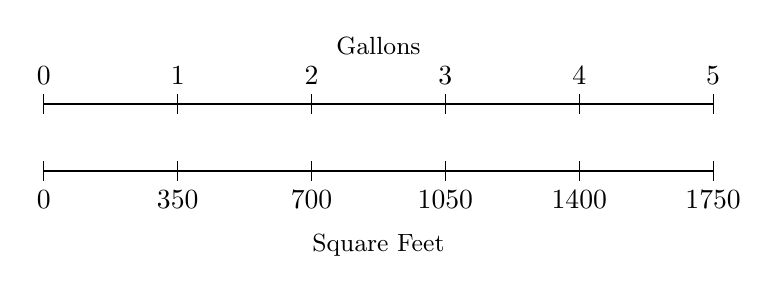
\begin{tikzpicture}[scale=0.85]
  \draw[thick] (0,0.5) -- (10,0.5);
  \draw[thick] (0,-0.5) -- (10,-0.5);
  \foreach \x/\lab in {0/0, 2/1, 4/2, 6/3, 8/4, 10/5}
    \draw (\x,0.35) -- (\x,0.65) node[above]{$\lab$};
  \node[above] at (5,1.1) {\small Gallons};
  \foreach \x/\lab in {0/0, 2/350, 4/700, 6/1050, 8/1400, 10/1750}
    \draw (\x,-0.35) -- (\x,-0.65) node[below]{$\lab$};
  \node[below] at (5,-1.3) {\small Square Feet};
\end{tikzpicture}
\end{center}

A room has $2{,}100$ sq ft of wall. Estimate the number of gallons needed.
\end{questionText}
\choiceA{$5$}
\choiceB{$6$}
\choiceC{$7$}
\choiceD{$8$}
\correctAnswer{B}
\explanation{Rate: $350$ sq ft per gallon. Gallons: $2{,}100 \div 350 = 6$.}
\end{practiceQuestion}

% --- Graphical Short Answer Questions (3) ---

\begin{practiceQuestion}{m-1-6-q25}{gsa}
\begin{questionText}
The table below shows typing speeds.

\begin{center}
\begin{tabular}{|c|c|}
\hline
\textbf{Minutes} & \textbf{Words Typed} \\
\hline
$3$ & $156$ \\
$5$ & $260$ \\
$8$ & $416$ \\
$12$ & $?$ \\
\hline
\end{tabular}
\end{center}

How many words will be typed in $12$ minutes?
\end{questionText}
\correctAnswer{$624$}
\explanation{Rate: $156 \div 3 = 52$ words per minute. For $12$ min: $52 \times 12 = 624$ words.}
\end{practiceQuestion}

\begin{practiceQuestion}{m-1-6-q26}{gsa}
\begin{questionText}
The graph below shows two streaming services' monthly data usage.

\begin{center}
\begin{tikzpicture}[scale=0.5]
  \draw[step=1,gray!20,thin] (0,0) grid (8,10);
  \draw[thick,->] (0,0) -- (8.5,0) node[right]{\small Hours};
  \draw[thick,->] (0,0) -- (0,10.5) node[above]{\small GB};
  \foreach \x in {1,...,8} \draw (\x,0.1) -- (\x,-0.1) node[below]{\tiny \x};
  \foreach \y in {2,4,6,8,10} \draw (0.1,\y) -- (-0.1,\y) node[left]{\tiny \y};
  \draw[thick,funGreen] (0,0) -- (8,6);
  \draw[thick,funOrange] (0,0) -- (8,4);
  \fill[funGreen] (4,3) circle (3pt);
  \fill[funOrange] (4,2) circle (3pt);
  \node[funGreen,right] at (8.1,6) {\tiny Service A};
  \node[funOrange,right] at (8.1,4) {\tiny Service B};
\end{tikzpicture}
\end{center}

How many more GB does Service A use than Service B in $12$ hours?
\end{questionText}
\correctAnswer{$3$ GB}
\explanation{Service A: from $(4, 3)$, rate $= \frac{3}{4} = 0.75$ GB/hr. In $12$ hrs: $0.75 \times 12 = 9$ GB. Service B: from $(4, 2)$, rate $= \frac{2}{4} = 0.5$ GB/hr. In $12$ hrs: $0.5 \times 12 = 6$ GB. Difference: $9 - 6 = 3$ GB.}
\end{practiceQuestion}

\begin{practiceQuestion}{m-1-6-q27}{gsa}
\begin{questionText}
The table shows the length and cost of lumber.

\begin{center}
\begin{tabular}{|c|c|}
\hline
\textbf{Length (ft)} & \textbf{Cost} \\
\hline
$6$ & $\$5.10$ \\
$8$ & $\$6.80$ \\
$10$ & $\$8.50$ \\
$14$ & $?$ \\
\hline
\end{tabular}
\end{center}

What is the cost of a $14$-foot piece of lumber?
\end{questionText}
\correctAnswer{$\$11.90$}
\explanation{Find the unit rate: $5.10 \div 6 = \$0.85$ per foot. Verify: $0.85 \times 8 = \$6.80$ ✓, $0.85 \times 10 = \$8.50$ ✓. For $14$ ft: $0.85 \times 14 = \$11.90$.}
\end{practiceQuestion}
